\documentclass[twocolumn]{preport}
\usepackage[dvipdfmx]{graphicx}
\graphicspath{{figs/}}
\usepackage{enumitem}
\usepackage{subcaption}

\title{等身大ヒューマノイドにおける道具操作技能の獲得に関する研究}
\author{東京大学工学部 機械情報工学科 03180266 河村洋一郎 指導教員 稲葉雅幸教授 岡田慧教授\\
  キ ーワ ード : humanoid, tool manipulation, force control, demonstration, reinforcement learning}

\begin{document}

\pagestyle{empty}
\maketitle
\thispagestyle{empty}
\sloppy

\section{本研究の背景と課題}
%% 等身大ヒューマノイドの家庭環境での幅広い活躍が未だ実現されていない理由の一つに,ハードウェアや計算機の性能等の設計上の仕様の限界から活動範囲が決まってしまうことが挙げられる.
道具の活用は等身大ヒューマノイドの活動幅を広げる一つの道筋であり,特に人を模倣した等身大ヒューマノイドは道具操作技能を獲得できることにより多くの恩恵を受けられることが期待されるが,真にこの恩恵を受けるためには道具を使いこなす能力,技能を獲得する必要がある.
道具操作技能はモデル化が難しいタスクに対して力加減の調整をする能力であり,反復試行的な学習によるアプローチが有効であるが,
(i)実ロボットによる大量データ確保の困難
(ii)報酬定義の困難
(iii)教示時の行動推定の必要性
,といった課題が存在する.
\vspace*{-8pt}
\section {本研究での取り組み}
(i)解決のために強化学習に教示を併用する.ロボットでの教示併用に関する先行研究では教示を事前に与え初期化に用いている\cite{kober2009learning}が,本研究ではタスクを反復試行する最中に報酬を監視することによって,失敗が連続し報酬が低迷している時にロボットが能動的に教示を要請する能動的教示要請法(A)を提案する.

(ii)解決法の一つにデモンストレーションから報酬関数を推定する逆強化学習~\cite{gao2012survey}が挙げられるが,報酬関数の推定と行動戦略の獲得を同時に行うため学習に時間を要する.そこで本研究では,人のデモンストレーションに近いなら報酬を高くするように報酬関数を定める手法(B)を提案する.

(iii)解決のために経験を蓄積することによりタスクに関する物理モデルを学習し,学習した物理モデルを用いて教示時の教師の行動を推定することでヒューリスティックな行動推定より質の高い教示データを獲得する教示再現行動推定(C)を提案する.

以上を統合したシステムの全体像をFig.1に示す.
\begin{figure}[tbh]
  \begin{center}
    \begin{minipage}{1.0\columnwidth}
      \includegraphics[width=1.0\columnwidth]{finale.png}
      \caption{General view of learning system.}
    \end{minipage}
    \begin{minipage}{1.0\columnwidth}
    \end{minipage}
    \label{figure:cartpole}
  \end{center}
\end{figure}
\vspace*{-15pt}

\vspace*{-5pt}
\subsection{倒立振子制御学習による有効性確認}
シミュレータ上で倒立振子制御を学習させた結果をFig.2に示す.Fig.2-(a)から既存手法Deep Q-network~\cite{mnih2015human} (以下DQN,青色)より(A)による学習(橙色)の方が報酬の上昇が早く,(C)での教示再現行動推定の正答率も経験の蓄積とともに上昇している(Fig.2-(b))ことから,手法(A) (B)の有効性が確認された.
\vspace*{-20pt}

\begin{figure}[htbp]
  \begin{minipage}{0.49\hsize}
    \begin{center}
      \includegraphics[width=1.00\columnwidth]{standing_time.png}
      \subcaption{}
    \end{center}
    \label{fig:one}
  \end{minipage}
  \begin{minipage}{0.49\hsize}
    \begin{center}
      \includegraphics[width=1.00\columnwidth]{demonstraion.png}
      \subcaption{}
    \end{center}
    \label{fig:two}
  \end{minipage}
  \caption{(a) Method (A) outperforms DQN. \ (b) Accuracy for action estimation increases.}
\end{figure}


\section{のこぎりとかんな技能の獲得}

のこぎり技能もかんな技能もロボットの動作は予め計算し,動作を実行する最中の力加減の調整を提案手法で獲得した.能動的教示要請(A)は反復学習中にロボット自ら教示を必要とすることを発話により伝えることで実行した(Fig.1左下).のこぎり動作に対する報酬(B)は,人のデモンストレーション時の音を計測しその音に近いかを判別することで決定した(Fig.1右上).かんな動作の成功/失敗は人が目視で判断することにより行った.学習の結果,のこぎりとかんな技能について経験の蓄積とともに(C)の教示行動推定の正答率が上昇する様子が見られた.
のこぎり技能獲得について,DQNと手法(A)との比較を行った結果、手法(A)の方が早期に報酬が増加した.かんな動作は学習により,成功率が上昇した.Fig.3はかんな技能を学習後に目標接触力(赤矢印)を調整している様子である.
\vspace*{-10pt}
%% \begin{figure}[tbh]
%%   \begin{center}
%%     \begin{minipage}{1.0\columnwidth}
%%       \begin{center}
%%       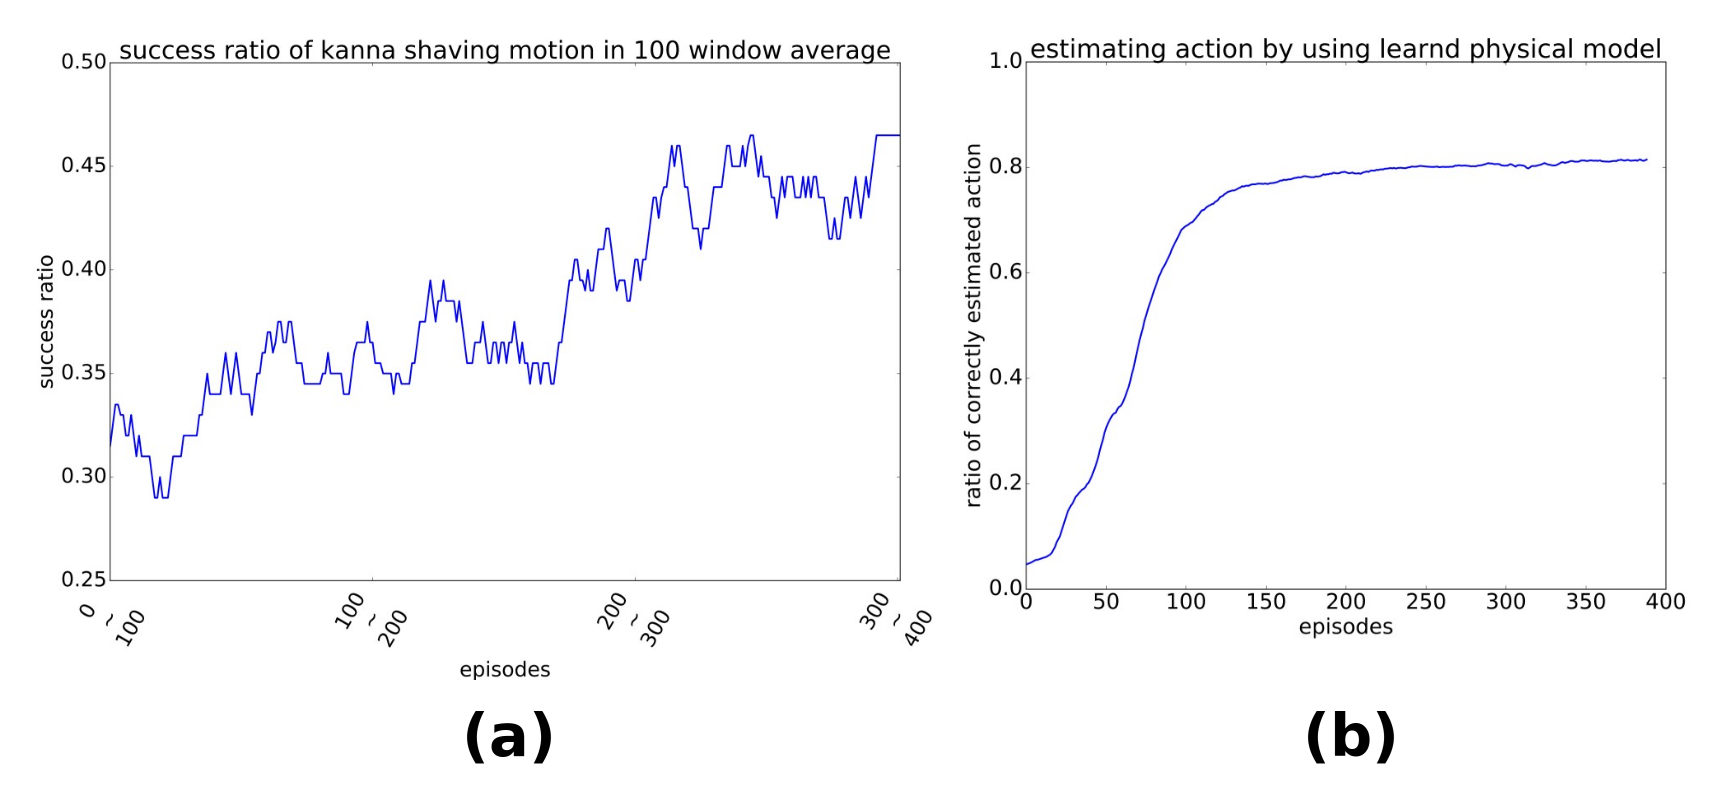
\includegraphics[width=0.6\columnwidth]{kannna_result.pdf}
%%       \caption{The humanoid robot actively requeseting human to teach.}
%%     \end{center}
%%     \end{minipage}
%%     \label{figure:kannna_result}
%%   \end{center}
%% \end{figure}

\begin{figure}[tbh]
  \label{figure:kanna_motion}
  \begin{minipage}{1.0\columnwidth}
    \begin{center}
      \includegraphics[width=0.8\columnwidth]{kannna_short}
      \caption{The humanoid robot manipulates a kanna.}
    \end{center}
    \end{minipage}
\end{figure}
\vspace*{-20pt}
\section{結論}
等身大ヒューマノイドHRP2-JSKNTSでの,のこぎり技能とかんな技能の獲得を通じ,能動的教示要請,デモンストレーションに基づく報酬関数設計,教示再現行動推定が,力調整能力を要する道具操作技能の効率的な学習のために有効であることを確認した.



%% \section{倒立振子制御学習による有効性確認}
%% シミュレータを用いた倒立振子学習に(i)(iii)の手法を
\bibliographystyle{junsrt}
\bibliography{p-report}

\end{document}

